\begin{Answer}{9}
		\begin{enumerate}[a),leftmargin=*]
			\i Lập bảng thống kê số lượng các bạn yêu thích mỗi màu áo đồng phục lớp.
			\begin{center}
				\begin{tabular}{|c|c|c|c|c|c|c|}
					\hline
						Màu áo&	Xanh lá&	Hồng&	Trắng&	Tím&	Đen&	Vàng\\
						\hline
					Số học sinh& 5&9&4&5&2&5\\	
					\hline
				\end{tabular}
			\end{center}
			\i Biểu đồ cột biểu thị số lượng các bạn yêu thích mỗi màu áo đồng phục lớp.
			\begin{figure}[H]
				\centering
				\vspace*{-5pt}
				\captionsetup{labelformat= empty, justification=centering}
				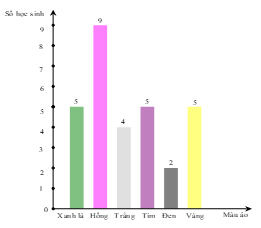
\includegraphics[width=0.5\linewidth]{9}
				\vspace*{-10pt}
			\end{figure}
		\end{enumerate}
	
\end{Answer}
\begin{Answer}{10}
		\begin{enumerate}[a),leftmargin=*]
			\i Bảng thống kê biểu diễn số lượng nhân viên sử dụng mỗi loại phương tiện đi làm.
			\begin{center}
				\begin{tabular}{|c|c|c|c|c|}
					\hline
					Loại phương tiện&	Xe buýt&	Xe đạp&	Xe máy&	Ô tô cá nhân\\
					\hline
					Số nhân viên& 35 &5&20&7\\
					\hline
				\end{tabular}
			\end{center}	
			\i Biểu đồ cột biểu diễn số lượng nhân viên sử dụng mỗi loại phương tiện đi làm
			\begin{figure}[H]
				\centering
				\vspace*{-5pt}
				\captionsetup{labelformat= empty, justification=centering}
				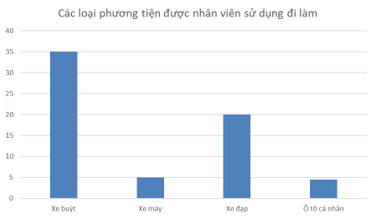
\includegraphics[width=0.5\linewidth]{10}
				\vspace*{-10pt}
			\end{figure}
		\end{enumerate}
	
\end{Answer}
\begin{Answer}{11}
		\begin{enumerate}[a),leftmargin=*]
			\i	Bảng trên có tên là bảng điều tra.\\
			Bảng thống kê:
			\begin{center}
				\begin{tabular}{|c|c|c|c|c|}
					\hline
					Tên môn học&	T&	Đ&	NN&	V\\
					\hline
					Số học sinh yêu thích&	15&	3&	9&	8\\
					\hline
				\end{tabular}
			\end{center}
			\i	Biểu đồ minh họa:
			\begin{figure}[H]
				\centering
				\vspace*{-5pt}
				\captionsetup{labelformat= empty, justification=centering}
				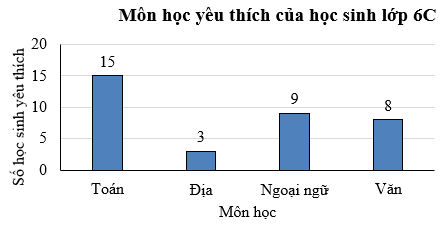
\includegraphics[width=0.5\linewidth]{11}
				\vspace*{-10pt}
			\end{figure}
			Qua biểu đồ trên ta thấy các bạn học sinh lớp $6C$ yêu thích nhất môn Toán.
		\end{enumerate}
	
\end{Answer}
\begin{Answer}{12}
		\begin{enumerate}[a),leftmargin=*]
			\i Ta có: ${\text{ƯCLN}}(32,16,20,44) = 4$\\
			Chọn mỗi biểu tượng  ứng với 4 học sinh mượn sách thư viện, ta có biểu đồ tranh sau
			\begin{center}
				\begin{tabular}{|l|l|}
					\hline
					Thứ hai&	\\
					\hline
					Thứ ba	&	\\
					\hline
					Thứ năm&	\\
					\hline
					Thứ sáu	&	\\
					\hline
				\end{tabular}
			\end{center}
			\i Vào thứ sáu học sinh đến thư viện trường mượn sách đọc nhiều nhất, thứ ba học sinh mượn sách ít nhất.
			
		\end{enumerate}
	
\end{Answer}
\begin{Answer}{13}
		Thiếu
	
\end{Answer}
\begin{Answer}{14}
		\begin{enumerate}[a),leftmargin=*]
			\i 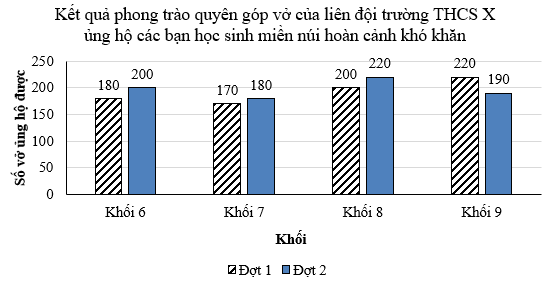
\includegraphics[width=0.5\linewidth]{12}
			\i Đợt 2 quyên góp nhận được sự ủng hộ của các bạn nhiều hơn.
		\end{enumerate}
	
\end{Answer}
\begin{Answer}{15}
		\begin{enumerate}[a),leftmargin=*]
			\i Chọn biểu đồ cột và vẽ như sau:
			\begin{figure}[H]
				\centering
				\vspace*{-5pt}
				\captionsetup{labelformat= empty, justification=centering}
				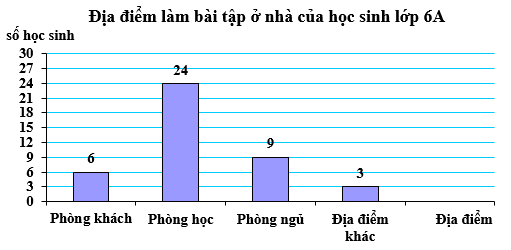
\includegraphics[width=0.5\linewidth]{13}
				\vspace*{-10pt}
			\end{figure}
			\i Lớp $6A$ có số học sinh là $6 + 24 + 9 + 3 = 42$  (học sinh).\\
			Theo em ở nhà các bạn học sinh lớp $6A$ hay làm bài tập ở phòng học nhất.
		\end{enumerate}
	
\end{Answer}
\begin{Answer}{16}
		\begin{enumerate}[a),leftmargin=*]
			\i Vì số bộ đồ chơi cắt hoa quả bố mẹ bạn An đã bán vào ngày chủ nhật đó là 6 bộ, trên biểu đồ ứng có 2 biểu tượng nên mỗi biểu tượng  ứng với 3 bộ đồ chơi đã bán được.
			\i Tổng số bộ đồ chơi đã bán trong ngày chủ nhật là: $\left( {5 + 3 + 3 + 2 + 8} \right).3 = 63$  (bộ)
			\i Đồ chơi Pop It được bố mẹ An bán ra nhiều nhất trong ngày chủ nhật.
			\i Bảng thống kê số đồ chơi bán được trong ngày chủ nhật của cửa hàng:
			\begin{center}
				\begin{tabular}{|l|c|}
					\hline
					&Số đồ chơi đã bán\\
					\hline
					Rubik&	15\\
					\hline
					Ô tô điều khiển&	9\\
					\hline
					Lego&	9\\
					\hline
					Bộ đồ chơi cắt hoa quả&	6\\
					\hline
					Pop It&	24\\
					\hline
				\end{tabular}
			\end{center}
		\end{enumerate}
	
\end{Answer}
\begin{Answer}{17}
		\begin{enumerate}[a),leftmargin=*]
			\i Số học sinh giỏi Toán của lớp $6E$ nhiều nhất: có 20 bạn. Số học sinh giỏi Toán của lớp 6A ít nhất: 9 bạn
			\i Số học sinh giỏi Ngữ văn của lớp $6D$ nhiều nhất: có 17 bạn. Số học sinh giỏi Ngữ văn của lớp 6A ít nhất: 7 bạn.
			\i Số học sinh giỏi Toán của lớp $6E$ chiếm số phần trăm trong tổng số học sinh giỏi môn Toán của cả 5 lớp là
			\[\dfrac{{20}}{{9 + 10 + 15 + 16 + 20}}.100\%  = 28,6\%\]
			\i Số học sinh giỏi Ngữ văn của lớp $6A$ chiếm số phần trăm trong tổng số học sinh giỏi môn Toán của cả 5 lớp là
			\[\dfrac{7}{{7 + 13 + 14 + 17 + 12}}.100\%  = 11,11\%\]
			\i Bạn Nam nói lớp $6D$ có sĩ số là 34 học sinh có thể chưa đúng vì: trong lớp có thể có học sinh không giỏi môn Toán, môn Ngữ văn và có thể có học sinh giỏi cả 2 môn Toán và Ngữ văn.
		\end{enumerate}
	
\end{Answer}
\begin{Answer}{18}
		\begin{enumerate}[a),leftmargin=*]
			\i Số lượng trong bảng số liệu đã cho chênh lệch nhau rất lớn nên khi vẽ biểu đồ khá khó khăn.
			\i Vì tính chất các mức độ khác nhau, "không ý kiến" khác rất nhiều với việc  ``có bày tỏ ý kiến của mình" nên không thể ghép dòng với nhau. Hợp lý hơn ta có thể ghép cột  ``Trí thức" với cột "Công nhân" vì trí thức có vẻ gần với công nhân hơn nông dân (đều ở khu vực thành thị). Như vậy ta có bảng mới sau:
			\begin{center}
				\begin{tabular}{|l|c|c|}
					\hline
					&Công nhân và trí thức&	Nông dân\\
					\hline
					Tăng&	120&	300\\
					\hline
					Như cũ&	230&	400\\
					\hline
					Giảm&	55&	80\\
					\hline
					Không ý kiến&	34&	70\\
					\hline
				\end{tabular}
			\end{center}
		\end{enumerate}
		\begin{figure}[H]
			\centering
			\vspace*{-5pt}
			\captionsetup{labelformat= empty, justification=centering}
			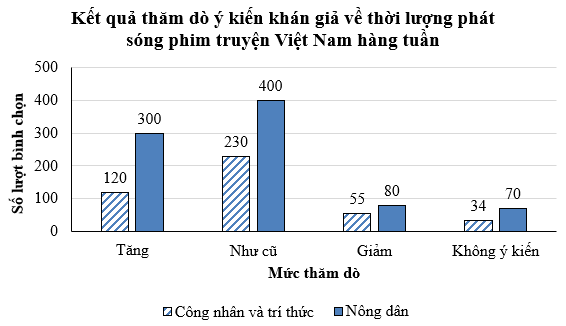
\includegraphics[width=0.5\linewidth]{14}
			\vspace*{-10pt}
		\end{figure}
	
\end{Answer}
